% Author Name: José Areia 
% Author Contact: jose.apareia@gmail.com
% Version: 2.2.13 - 2026/01/06
% Public Repository: https://github.com/joseareia/ipleiria-thesis
% Wiki/Getting Help: https://github.com/joseareia/ipleiria-thesis/wiki

%%% Document Options %%%
\documentclass[
    language=vietnamese,
    school=hcmus,
    docstage=final,
    media=screen,
    bookprint=false,
    linkcolor=blue!55!black,
    chapterstyle=fancy,
    coverstyle=classic,
    aiacknowledgement=false,
    listprefix=false
]{ReportThesis} % Refer to the Wiki for a list of available options.

%%% Document Version %%%
\DocumentVersion{1.0.0} % Required only if the 'docstage' is set to 'working'.

%%% Document Metadata %%%
% First Author (Mandatory)
\FirstAuthor{Nguyễn Đỗ Bảo}
\FirstAuthorNumber{23127026}

% Second Author (Optional)
% \SecondAuthor{Jane Smith}
% \SecondAuthorNumber{2230456}

% Third Author (Optional)
% \ThirdAuthor{July Smith}
% \ThirdAuthorNumber{2230457}

% Supervisor (Mandatory)
\Supervisor{Lê Nhựt Nam}
\SupervisorMail{le.nhut.nam@ipleiria.pt}
% Please provide: [Current Title, Affiliation]
\SupervisorTitle{Khoa Công nghệ Thông tin} 

% Co-Supervisor (Optional)
% \CoSupervisor{Steve Smith}
% \CoSupervisorMail{steve.smith@ipleiria.pt}
% \CoSupervisorTitle{Associate Professor, Polytechnic of Leiria}

% Second Co-Supervisor (Optional)
% \SecCoSupervisor{Shak Smith}
% \SecCoSupervisorMail{shak.smith@ipleiria.pt}
% \SecCoSupervisorTitle{Associate Researcher, Computer Science \& Communication Research Centre}

% Title (Mandatory)
\Title{Đồ án 2 - Khai Thác Tập Phổ Biến}

% Subtitle (Mandatory)
\Subtitle{Nghiên cứu, Cài đặt, và Đánh giá}

% University (Mandatory)
\University{Đại học Quốc gia Thành phố Hồ Chí Minh}

% School (Mandatory)
\School{Trường Đại học Khoa học Tự nhiên}

% Department (Mandatory)
\Department{Khoa Công nghệ Thông tin}

% Degree (Mandatory)
\Degree{}

% Course (Optional)
\Course{CSC14004 - Khai thác Dữ liệu và Ứng dụng}

% Thesis Theme (Mandatory)
% \ThesisType{Dissertation/Project/Internship \\ \textcolor{blue}{(Erase the Non-Essential)}}

% Local & Date (Mandatory)
\Date{Hồ Chí Minh, Tháng 4/2026}

% Academic Year 
\AcademicYear{2025/2026}

\begin{document}

%%% Front Matter %%%
\include{Matter/00-Cover}
\include{Matter/01-Front-Page}

%%% Copyright Statement %%%
% \include{Matter/02-Copyright}

%%% Roman Numeration %%%
\pagenumbering{roman}

%%% Acknowledgements %%%
% \include{Matter/03-Acknowledgements}

%%% Abstract %%%
% \include{Chapters/00-Abstract}

%%% AI Acknowledgement %%%
% \include{Matter/04-AI}

%%% Table of Contents, List of Figures and List of Tables %%%
\bookmarktocentry\tableofcontents
\listoffigures
\listoftables

%%% Print: Glossary and Acronyms %%%
% \glossarytoc\printnormalglossary
% \acronymtoc\printacronymglossary
% \symboltoc\printsymbolglossary

%%% Arabic Numeration %%%
\pagenumbering{arabic}

%%% Chapters (**Insert Yours Here**) %%%
\chapter[Nền tảng lý thuyết]{Nền tảng lý thuyết}
\label{cp:theoretical-foundation}

\section{Bài toán khai thác tập phổ biến}

\subsection{Cơ sở dữ liệu giao dịch (transaction database)}
\textbf{Cơ sở dữ liệu giao dịch} (CSDL) $\mathcal{D}$ bao gồm một tập hợp các giao dịch $T$, trong đó mỗi giao dịch chứa một tập hợp các hạng mục không rỗng (\textit{itemset}) $\mathcal{I} = \{i_1, i_2, \ldots, i_m\}$ sao cho $T \subseteq \mathcal{I}$ và được gán với một định danh giao dịch duy nhất (TID). Ta nói giao dịch $T$ chứa $X$ (với $X$ là tập các hạng mục trong $\mathcal{I}$), nếu $X \subseteq T$.

\subsection{Độ hỗ trợ (support)}
\textbf{Độ hỗ trợ} (\textit{support}) của một tập hạng mục $X$ là phần trăm số lượng giao dịch có chứa $X$ trong cơ sở dữ liệu giao dịch $\mathcal{D}$, có thể được định nghĩa bằng (\ref{eq:equation-1-1}):
\begin{equation}
    \label{eq:equation-1-1}
    \textit{sup}(X) = \frac{|\{T \mid X \subseteq T \land T \in \mathcal{D}\}|}{|\mathcal{D}|}
\end{equation}
    
Có hai cách để biểu diễn độ hỗ trợ là \textbf{độ hỗ trợ tuyệt đối} (\textit{absolute support} hay \textit{support count}) và \textbf{độ hỗ trợ tương đối} (\textit{relative support}).

\textbf{Độ hỗ trợ tuyệt đối} của một tập hạng mục $X$ là số lượng giao dịch trong CSDL chứa $X$, được định nghĩa bằng:
\begin{equation}
    \label{eq:equation-1-2}
    \textit{support\textunderscore count}(X) = |\{T \mid X \subseteq T \land T \in \mathcal{D}\}|
\end{equation}

\textbf{Độ hỗ trợ tương đối} của một tập hạng mục $X$ là tỷ lệ giữa độ hỗ trợ tuyệt đối của $X$ và tổng số giao dịch trong CSDL, biểu diễn bằng (\ref{eq:equation-1-1}).

\subsection{Tập phổ biến (frequent itemset)}
Ta nói $X$ là \textbf{tập phổ biến} khi $\textit{sup}(X) \geq $ \textit{minsup} trong đó \textit{minsup} là ngưỡng hỗ trợ tối thiểu được định trước. Một tập hạng mục chứa k hạng mục là một \textbf{k-itemset}. Tập hợp của các tập phổ biến k-itemset được ký hiệu là $L_k$.

\subsection{Tập đóng (closed itemset) và tập tối đại (maximal itemset)}
Tập hạng mục $X$ được gọi là \textbf{đóng} (\textit{closed}) trong tập dữ liệu $D$ nếu không tồn tại một siêu tập hợp (\textit{superitemset}) $Y$ (tức là, mọi phần tử của $X$ đều thuộc $Y$, nhưng tồn tại ít nhất một phần tử của $Y$ không thuộc $X$) nào chứa $X$ mà $Y$ có cùng số hỗ trợ (\textit{support count}) với $X$ trong $D$, hay nói cách khác:
\begin{equation}
    \label{eq:equation-1-3}
    \nexists Y \mid (X \subset Y) \land (\textit{sup}(X) = \textit{sup}(Y))
\end{equation}
Tập hạng mục $X$ là \textbf{tập phổ biến đóng} (\textit{closed frequent itemset}) khi thỏa mãn cả tính đóng và tính phổ biến.

Tập hạng mục $X$ được gọi là \textbf{tập tối đại} (\textit{maximal itemset}) trong tập dữ liệu $D$ nếu không tồn tại một siêu tập hợp $Y$ nào chứa $X$ trong $D$, hay nói cách khác:
\begin{equation}
    \label{eq:equation-1-4}
    \nexists Y \mid (X \subset Y)
\end{equation}
Tập hạng mục $X$ là \textbf{tập phổ biến tối đại} (\textit{maximal frequent itemset}) khi thỏa mãn cả tính tối đại và tính phổ biến.

Mối quan hệ giữa tập phổ biến (FI), tập phổ biến đóng (CFI), và tập phổ biến tối đại (MFI) được biểu diễn như sau: MFI $\subseteq$ CFI $\subseteq$ FI.

\subsection{Tính chất Apriori (downward closure)}
\textbf{Tính chất Apriori}: Tất cả các tập con không rỗng của một tập hạng mục phổ biến cũng phải là các tập phổ biến.

\textbf{Tính chất đơn điệu giảm (antimonotonicity)}: Nếu một tập hợp không vượt qua được một phép thử, thì tất cả các tập hợp cha của nó cũng sẽ không vượt qua được phép thử đó.

\textbf{Chứng minh}: Nếu một tập hạng mục $I$ không thỏa mãn điều kiện về độ hỗ trợ tối thiểu (\textit{minsup}), thì $I$ sẽ không phải là tập phổ biến (tức là $P(I) < \textit{minsup}$). Khi đó, nếu có một hạng mục $a$ được thêm vào $I$, thì tập hạng mục ($I \cup \{a\}$) sẽ không thể xuất hiện nhiều lần hơn $I$. Vả lại, có thể coi ($I \cup \{a\}$) là tập cha của $I$ (vì $I \subset (I \cup \{a\})$). Do đó, ($I \cup \{a\}$) cũng không thể là tập phổ biến (do $P(I \cup \{a\}) < \textit{minsup}$).

\section{Phân tích thuật toán AprioriTID}
Thuật toán tìm tập hạng mục lớn (\textit{large itemsets}) hoạt động lặp đi lặp lại qua nhiều lượt quét CSDL. Ở lượt đầu tiên, thuật toán đếm độ hỗ trợ (\textit{support}) của từng hạng mục để tìm các large 1-itemset. Ở các vòng tiếp theo, các large itemset từ vòng trước được dùng làm cơ sở sinh ra các tập ứng viên (\textit{candidate itemsets}). Thuật toán tiếp tục quét CSDL để đếm support cho ứng viên, lọc ra các large itemset mới và lặp lại quá trình này cho đến khi không tìm thêm được tập nào nữa.

\subsection{Ý tưởng cốt lõi}
Thuật toán Apriori tìm tập phổ biến thông qua quá trình sinh ứng viên và kiểm tra theo từng mức độ dài, trong đó các large k-itemset được sử dụng để khám phá các large (k+1)-itemset. Ý tưởng cốt lõi của AprioriTID dựa trên một biến thể tối ưu hóa gọi là giảm thiểu giao dịch (\textit{transaction reduction}). Nếu một giao dịch không chứa bất kỳ k-itemset phổ biến nào thì nó cũng không thể chứa bất kỳ (k+1)-itemset phổ biến nào khác. Do đó, ta loại bỏ các TID này và không cần xét đến chúng trong các lần quét CSDL ở các vòng lặp tiếp theo. Thay vì phải quét lại CSDL gốc nhiều lần, AprioriTID tạo ra một tập dữ liệu mã hóa trung gian, ký hiệu là $\overline{C}_k$ để lưu vết những ứng viên có mặt trong từng giao dịch. Ở các vòng lặp sau, tập $\overline{C}_k$ này có thể trở nên nhỏ hơn rất nhiều so với kích thước của CSDL gốc, giúp tiết kiệm đáng kể chi phí đọc đĩa (I/O).

Đầu tiên, tìm tập hợp 1-itemset phổ biến bằng cách đếm số lần xuất hiện của TID chứa 1-itemset, và thu thập những 1-itemset thỏa mãn minsup. Tập hợp kết quả được ký hiệu là $L_1$. Tiếp theo, $L_1$ được sử dụng để tìm $L_2$, tập hợp các 2-itemset phổ biến, được sử dụng để tìm $L_3$, và cứ thế tiếp tục cho đến khi không còn k-itemset phổ biến nào được tìm thấy nữa.

Các thuật toán đi trước như AIS hay SETM sinh các tập ứng viên ngay tức thì (on-the-fly) bằng cách đọc từng giao dịch và mở rộng các tập phổ biến có trong giao dịch đó. Cách này tạo ra vô số ứng viên dư thừa, dẫn đến lãng phí tài nguyên. AprioriTID khắc phục điều này bằng cách sinh ứng viên một cách độc lập thông qua việc nối các tập phổ biến bước trước, tạo ra tập ứng viên nhỏ hơn rất nhiều.


\subsection{Cấu trúc dữ liệu chính}
AprioriTID sử dụng một cấu trúc dữ liệu mảng tuần tự đặc trưng là tập $\overline{C}_k$.  Mỗi phần tử trong $\overline{C}_k$ đại diện cho một giao dịch, có định dạng: {$\langle \text{TID},\{X_k\}\rangle$}, trong đó $X_k$ là k-itemset xuất hiện trong TID. Nếu một giao dịch không chứa bất kỳ ứng viên nào, nó sẽ không có mục (\textit{entry}) tương ứng trong $\overline{C}_k$.

Lấy ví dụ minh họa CSDL $\mathcal{D}$ ở \autoref{fig:example-1} với TID $101$ chứa các mục: \{1, 2, 3, 4\}. Ngưỡng \textit{minsup} = 2.

\begin{itemize}
    \item Ở bước $k=1$, $\overline{C}_1$ sẽ là: $\langle$ 101, \{\{1\}, \{2\}, \{3\}, \{4\}\} $\rangle$.
    \item Ở bước $k=2$, tập ứng viên $C_2$ chứa \{1, 2\}, \{1, 4\}, \{1, 5\},... (lưu ý mục \{3\} không đạt minsup ở $L_1$ nên các tập chứa \{3\} không xuất hiện trong $C_2$). Vì TID 101 chứa các tổ hợp con hợp lệ nằm trong $C_2$ là \{1, 2\}, \{1, 4\}, \{2, 4\}, nên $\overline{C}_2$ cho TID 101 sẽ là: $\langle$ 101, \{\{1, 2\}, \{1, 4\}, \{2, 4\}\} $\rangle$.
    \item Ở bước $k=3$, tập ứng viên $C_3$ là \{\{1, 2, 4\}, \{1, 4, 5\}\}. Giao dịch 101 chỉ chứa tổ hợp \{\{1, 2, 4\}\} có mặt trong $C_3$, nên $\overline{C}_3$ cho TID 101 sẽ là: $\langle$ 101, \{\{1, 2, 4\}\} $\rangle$.
    \item Ở bước $k=4$, vì $L_3$ = \{\{1, 2, 4\}, \{1, 4, 5\}\} không có hai phần tử nào trùng tiền tố độ dài 2, nên hàm apriori-gen trả về $C_4 = \emptyset$ và vòng lặp kết thúc.
\end{itemize}

\subsection{Mã giả (Pseudocode)}
\begin{figure}[!ht]
\centering
\begin{minipage}{\linewidth}
\noindent\textbf{Thuật toán AprioriTID}

\noindent\textbf{Input:}
\begin{itemize}[nosep,leftmargin=2em,topsep=2pt]
    \item $\mathcal{D}$: cơ sở dữ liệu giao dịch;
    \item \textit{minsup}: ngưỡng độ hỗ trợ tối thiểu.
\end{itemize}
\noindent\textbf{Output:} $L$, tập các itemset phổ biến trong $\mathcal{D}$.

\noindent\textbf{Method:}
\begin{algorithmic}[1]
\State $L_1 \gets \{\text{các 1-itemset phổ biến}\}$
\State $\overline{C}_1 \gets \mathcal{D}$
\For{$k \gets 2$; $L_{k-1} \neq \emptyset$; $k{+}{+}$}
    \State $C_k \gets \text{apriori-gen}(L_{k-1})$ \Comment{sinh ứng viên mới}
    \State $\overline{C}_k \gets \emptyset$
    \ForAll{phần tử $t \in \overline{C}_{k-1}$}
        \State $C_t \gets \{c \in C_k \mid (c - c[k]) \in t.\text{set-of-itemsets} \land (c - c[k-1]) \in t.\text{set-of-itemsets}\}$
        \ForAll{ứng viên $c \in C_t$}
            \State $c.\text{count} \gets c.\text{count} + 1$
        \EndFor
        \If{$C_t \neq \emptyset$}
            \State $\overline{C}_k \gets \overline{C}_k \cup \{\langle t.\text{TID}, C_t \rangle\}$
        \EndIf
    \EndFor
    \State $L_k \gets \{c \in C_k \mid c.\text{count} \geq \textit{minsup}\}$
\EndFor
\State \Return $L = \bigcup_k L_k$
\end{algorithmic}

\vspace{0.6em}
\noindent\textbf{procedure apriori-gen}($L_{k-1}$: tập phổ biến $(k{-}1)$-itemset)\textbf{:}
\begin{algorithmic}[1]
\ForAll{itemset $l_1 \in L_{k-1}$}
    \ForAll{itemset $l_2 \in L_{k-1}$}
        \If{$(l_1[1] = l_2[1]) \land \ldots \land (l_1[k{-}2] = l_2[k{-}2]) \land (l_1[k{-}1] < l_2[k{-}1])$}
            \State $c \gets l_1 \bowtie l_2$ \Comment{bước join: sinh ứng viên}
            \If{has\_infrequent\_subset($c, L_{k-1}$)}
                \State \textbf{delete} $c$ \Comment{bước prune: loại ứng viên không đạt}
            \Else
                \State thêm $c$ vào $C_k$
            \EndIf
        \EndIf
    \EndFor
\EndFor
\State \Return $C_k$
\end{algorithmic}

\vspace{0.6em}
\noindent\textbf{procedure has\_infrequent\_subset}($c$: ứng viên $k$-itemset; $L_{k-1}$: tập phổ biến $(k{-}1)$-itemset)\textbf{:}
\begin{algorithmic}[1]
\ForAll{$(k{-}1)$-subset $s$ của $c$}
    \If{$s \notin L_{k-1}$}
        \State \Return TRUE
    \EndIf
\EndFor
\State \Return FALSE
\end{algorithmic}
\end{minipage}
\caption{Thuật toán AprioriTID tìm tập phổ biến dựa trên sinh ứng viên.}
\label{fig:AprioriTid}
\end{figure}

\textbf{Giải thích mã giả:}
\begin{enumerate}
    \item (1) Tìm tập hợp các tập phổ biến có kích thước bằng 1 ($L_1$);
    \item (2) Khởi tạo $\overline{C}_1 = \mathcal{D}$. Mỗi item trong mỗi giao dịch được xem là một tập 1-itemset, tạo thành định dạng $\langle \text{TID}, \text{tập các 1-itemset} \rangle$;
    \item (3) Bắt đầu vòng lặp tìm các tập phổ biến kích thước $k$ ($k\geq2$). Vòng lặp này sẽ tiếp tục cho đến khi $L_{k-1} = \emptyset$;
    \item (4) Sinh ra tập các ứng viên kích thước $k$ ($C_k$) từ tập phổ biến $L_{k-1}$. Hàm apriori-gen dùng để sinh ra tập các ứng viên k-itemset $C_k$ từ tập phổ biến $L_{k-1}$;
    \item (5) Khởi tạo tập $\overline{C}_k$ rỗng;
    \item (6 - 11) Duyệt qua $\overline{C}_{k-1}$ để xác định và tăng biến đếm độ hỗ trợ cho các ứng viên trong $C_k$ thực sự xuất hiện trong mỗi giao dịch. Sau đó xây dựng $\overline{C}_k$, chỉ giữ lại những giao dịch có chứa ít nhất một ứng viên $k$-itemset;
    \item (12) Lọc ra tập phổ biến $L_k$. Chỉ giữ lại những ứng viên trong $C_k$ có $\text{count} \geq \textit{minsup}$;
    \item (14) Hợp nhất toàn bộ các tập $L_k$ là danh sách tất cả các itemset phổ biến trong CSDL.
\end{enumerate}

Hàm \texttt{apriori-gen} nhận đầu vào là $L_{k-1}$, tức là tập hợp tất cả các tập large $(k{-}1)$-itemset, và trả về một tập hợp gồm các large $k$-itemset. Nó gồm hai bước: (1) \textbf{join} — hợp $L_{k-1}$ với chính nó để sinh ra các tập ứng viên $C_k$; và (2) \textbf{prune} — tỉa tất cả các ứng viên $c \in C_k$ nếu tồn tại bất kỳ $(k{-}1)$-itemset nào của $c$ không nằm trong $L_{k-1}$ (xem thủ tục \texttt{has\_infrequent\_subset} trong \autoref{fig:AprioriTid}).

Lấy ví dụ CSDL $\mathcal{D}$ ở \autoref{fig:example-1} có $L_2$: \{\{1 2\}, \{1 4\}, \{1 5\}, \{2 4\}, \{4 5\}\}. Bước join ghép các cặp có cùng item đầu tiên và item thứ hai theo thứ tự tăng dần: \{1 2\}$\bowtie$\{1 4\}, \{1 2\}$\bowtie$\{1 5\}, \{1 4\}$\bowtie$\{1 5\}, sinh ra $C_3$: \{\{1 2 4\}, \{1 2 5\}, \{1 4 5\}\}. Bước prune xóa \{1 2 5\} vì tập con \{2 5\} không nằm trong $L_2$. Do đó chỉ còn lại \{\{1 2 4\}, \{1 4 5\}\} ở $C_3$.

\subsection{Phân tích độ phức tạp}

\begin{table}[h]
\centering
\begin{tabular}{cl}
\hline
\textbf{Ký hiệu} & \textbf{Ý nghĩa} \\
\hline
$n$           & Số giao dịch trong CSDL $\mathcal{D}$ \\
$|I|$         & Số lượng hạng mục (item) phân biệt \\
$w$           & Độ rộng trung bình của một giao dịch \\
$k_{\max}$    & Độ dài tập phổ biến dài nhất \\
$|C_k|$       & Số ứng viên ở bước $k$ \\
$|L_k|$       & Số tập phổ biến ở bước $k$ \\
$|\overline{C}_k|$ & Tổng số cặp $\langle\text{TID}, \text{itemset}\rangle$ trong $\overline{C}_k$ \\
\textit{minsup} & Ngưỡng độ hỗ trợ tối thiểu \\
\hline
\end{tabular}
\caption{Các ký hiệu dùng trong phân tích độ phức tạp.}
\label{tab:complexity-notation}
\end{table}

\subsubsection{Phân rã chi phí theo từng bước}

\paragraph{Bước 1 — Khởi tạo.}
Thuật toán quét toàn bộ CSDL $\mathcal{D}$ một lần duy nhất để tính độ hỗ trợ
từng 1-itemset và khởi tạo $\overline{C}_1$. Độ phức tạp:
\begin{equation}
    \label{eq:equation-1-5a}
    T_{\text{init}} = O(n \cdot w)
\end{equation}

\paragraph{Bước 2 — Sinh ứng viên bằng \texttt{apriori-gen}.}
Hàm \texttt{apriori-gen} gồm hai pha con:
\begin{itemize}[nosep,topsep=2pt]
    \item \textit{Join:} duyệt mọi cặp $(p,q) \in L_{k-1} \times L_{k-1}$, mỗi phép so sánh tốn $O(k)$ để kiểm tra $k{-}2$ item đầu khớp và item cuối theo thứ tự:
    \begin{equation}
        \label{eq:equation-1-5b}
        T_{\text{join}}(k) = O\!\left(|L_{k-1}|^2 \cdot k\right)
    \end{equation}
    \item \textit{Prune:} với mỗi ứng viên $c \in C_k$, sinh $k$ tập con kích thước $(k{-}1)$ và kiểm tra thành viên trong $L_{k-1}$:
    \begin{equation}
        \label{eq:equation-1-5c}
        T_{\text{prune}}(k) = O\!\left(|C_k| \cdot k \cdot |L_{k-1}|\right)
    \end{equation}
\end{itemize}
Tổng chi phí \texttt{apriori-gen} tại bước $k$:
\begin{equation}
    \label{eq:equation-1-5d}
    T_{\text{gen}}(k) = O\!\left(|L_{k-1}|^2 \cdot k \;+\; |C_k| \cdot k \cdot |L_{k-1}|\right)
\end{equation}

\paragraph{Bước 3 — Đếm support qua $\overline{C}_k$.}
Đây là điểm then chốt phân biệt AprioriTID với Apriori cơ bản: thay vì quét lại $\mathcal{D}$, thuật toán duyệt cấu trúc trung gian $\overline{C}_{k-1}$. Với mỗi phần tử $t \in \overline{C}_{k-1}$, thuật toán xác định tập ứng viên $C_t$ có trong $t$, tăng $c.\text{count}$ cho mọi $c \in C_t$, rồi ghi $\langle t.\text{TID}, C_t \rangle$ vào $\overline{C}_k$ nếu $C_t \neq \emptyset$. Chi phí:
\begin{equation}
    \label{eq:equation-1-5e}
    T_{\text{count}}(k) = O\!\left(|\overline{C}_k| \cdot k\right)
\end{equation}
Khi $k$ tăng, $|\overline{C}_k|$ thường giảm nhanh do transaction reduction, nhỏ hơn rất nhiều so với chi phí $O(n \cdot |C_k|)$ nếu phải quét lại $\mathcal{D}$.

\paragraph{Tổng chi phí thời gian.}
Gộp cả ba bước:
\begin{equation}
    \label{eq:equation-1-5}
    T_{\text{total}} = O(n \cdot w)
    + \sum_{k=2}^{k_{\max}}
        \Bigl[
        |L_{k-1}|^2 \cdot k
        \;+\; |C_k| \cdot k \cdot |L_{k-1}|
        \;+\; |\overline{C}_k| \cdot k
        \Bigr].
\end{equation}

\subsubsection{Độ phức tạp thời gian theo trường hợp}

\paragraph{Trường hợp tốt nhất.}
Xảy ra khi dữ liệu thưa và \textit{minsup} cao: $|L_k|$ nhỏ, $k_{\max}$ nhỏ, và $|\overline{C}_k|$ giảm nhanh sau $k = 2$. Khi đó chi phí $T_{\text{count}}(k)$ chiếm ưu thế nhưng $\sum_k |\overline{C}_k| \ll n \cdot k_{\max}$, và thuật toán dừng sớm sau vài vòng lặp. Chi phí xấp xỉ:
\begin{equation}
    \label{eq:equation-1-6}
    T_{\text{best}} = O(n \cdot w + |L_1|^2 + |\overline{C}_2| \cdot 2)
\end{equation}
AprioriTID vượt trội so với Apriori chuẩn nhờ tránh được $k_{\max}$ lần quét lại $\mathcal{D}$.

\paragraph{Trường hợp trung bình.}
Trên CSDL giao dịch thực tế điển hình, số tập phổ biến có phân bố thưa dần theo $k$: $|L_k|$ đạt cực đại quanh $k = 2$ hoặc $k = 3$ rồi giảm dần, và $|\overline{C}_k|$ co lại nhanh ở các bước sau. Chi phí bị chi phối bởi vài vòng lặp đầu tiên:
\begin{equation}
    \label{eq:equation-1-7}
    T_{\text{avg}} = O\!\left(n \cdot w + \sum_{k=2}^{k_{\max}} |\overline{C}_k| \cdot k\right)
\end{equation}
với tổng $\sum_k |\overline{C}_k|$ thường chỉ là bội số hằng số của $n \cdot w$. Đây là chế độ hoạt động mà AprioriTID được thiết kế để tối ưu.

\paragraph{Trường hợp xấu nhất.}
Xảy ra khi dữ liệu \textbf{dày đặc} và \textit{minsup} thấp: gần như mọi itemset đều phổ biến, $|L_k|$ tăng theo hướng tổ hợp $\binom{|I|}{k}$, và $|\overline{C}_k|$ không co lại. Khi đó số ứng viên tối đa là $O(2^{|I|})$ và độ phức tạp thời gian trở thành \textit{hàm mũ} theo $|I|$:
\begin{equation}
    \label{eq:equation-1-8}
    T_{\text{worst}} = O\!\left(2^{|I|} \cdot |I|\right).
\end{equation}
Đây là giới hạn lý thuyết chung cho mọi thuật toán sinh-và-kiểm-tra (\textit{generate-and-test}) dựa trên Apriori.

\subsubsection{Độ phức tạp không gian}
\begin{table}[h!]
\centering
\begin{tabular}{lll}
\hline
\textbf{Cấu trúc} & \textbf{Không gian} & \textbf{Ghi chú} \\
\hline
CSDL gốc $\mathcal{D}$   & $O(n \cdot w)$        & Lưu trữ đầu vào \\
$C_k,\; L_k$ mỗi vòng   & $O(|C_k| \cdot k)$   & Tập ứng viên và tập phổ biến \\
$\overline{C}_k$ (đặc trưng AprioriTID) & $O(n \cdot |C_k|)$ & Lớn nhất ở $k = 2$, giảm dần \\
\hline
\end{tabular}
\caption{Độ phức tạp không gian của các cấu trúc chính.}
\label{tab:complexity-space}
\end{table}

\noindent Điểm đáng chú ý là $\overline{C}_k$ ở giai đoạn $k = 2$ có thể \textbf{lớn hơn} $\mathcal{D}$ gốc: mỗi giao dịch $w$ item ánh xạ thành $\binom{w}{2}$ cặp ứng viên, dẫn tới tăng \textit{bậc hai} theo $w$. Đây là điểm yếu bộ nhớ chính của AprioriTID so với Apriori tiêu chuẩn, đặc biệt rõ trên dữ liệu dày đặc (xem minh họa ở \autoref{cp:example}).

\subsubsection{Các yếu tố ảnh hưởng đến hiệu năng}
Ba yếu tố chính quyết định hiệu năng thực tế của AprioriTID:
\begin{itemize}[nosep,topsep=2pt]
    \item \textbf{Ngưỡng \textit{minsup}.} Yếu tố ảnh hưởng mạnh nhất. \textit{minsup} thấp làm $|L_k|$, $|C_k|$ và $|\overline{C}_k|$ tăng nhanh theo cấp số, kéo theo cả chi phí thời gian lẫn bộ nhớ. Ngược lại, \textit{minsup} cao giúp transaction reduction cắt tỉa $\overline{C}_k$ nhanh chóng, đưa thuật toán về gần trường hợp tốt nhất.
    \item \textbf{Kích thước và mật độ của CSDL.} Số giao dịch $n$ chỉ ảnh hưởng tuyến tính ở bước khởi tạo $O(n \cdot w)$. Ngược lại, \textit{mật độ} của dữ liệu (tỷ lệ item mỗi giao dịch chứa) mới là yếu tố then chốt: dữ liệu dày đặc (chess, mushroom) làm $|\overline{C}_2|$ phình to và $k_{\max}$ dài hơn, còn dữ liệu thưa (retail, T10I4D100K) giúp thuật toán hội tụ nhanh.
    \item \textbf{Độ rộng trung bình giao dịch $w$.} Ảnh hưởng \textit{bậc hai} lên kích thước $\overline{C}_2$ (mỗi giao dịch sinh $\binom{w}{2}$ cặp ứng viên) và ảnh hưởng tuyến tính lên bước khởi tạo. Giao dịch càng dài thì cả thời gian lẫn bộ nhớ cao điểm đều tăng.
\end{itemize}
\noindent Ba yếu tố này sẽ được kiểm chứng bằng thực nghiệm trong \autoref{cp:experiment-evaluation}.

\subsection{So sánh lịch sử}
Trong giai đoạn đầu của lĩnh vực khai phá tập phổ biến (FIM), các thuật toán tiên phong như AIS và SETM gặp nhiều hạn chế do phải sinh ứng viên "on-the-fly" (trên đường bay) trong quá trình đọc giao dịch và đòi hỏi việc rà quét, sắp xếp cơ sở dữ liệu gốc liên tục rất tốn kém. Sự ra đời của thuật toán Apriori và AprioriTID vào năm 1994 bởi R. Agrawal và R. Srikant đã tạo ra một bước ngoặt lớn khi giải quyết được những nhược điểm này. Điểm cải tiến mang tính lịch sử của AprioriTID là nó áp dụng hàm sinh ứng viên tiên nghiệm giúp thu hẹp không gian tìm kiếm, đồng thời sử dụng cấu trúc dữ liệu trung gian mã hóa ($\overline{C}_k$) để đếm độ hỗ trợ. Nhờ vậy, thuật toán không cần phải quét lại cơ sở dữ liệu gốc từ vòng lặp thứ hai trở đi, giúp giảm thiểu đáng kể chi phí truy xuất đĩa (I/O) so với các thuật toán tiền nhiệm.

Mặc dù là một bước tiến lớn, AprioriTID vẫn để lại một hạn chế cốt lõi: nó vẫn hoàn toàn phụ thuộc vào mô hình "sinh và kiểm tra" (generate-and-test), sinh ra vô số ứng viên nhỏ không cần thiết và dễ gây quá tải bộ nhớ khi xử lý các tập dữ liệu lớn. Để giải quyết bài toán này, các thế hệ thuật toán FIM sau đó đã thay đổi hoàn toàn cách tiếp cận. Nổi bật là thuật toán FP-Growth ra đời bằng cách áp dụng cấu trúc cây nén FP-tree kết hợp với chiến lược "chia để trị", giúp khai phá trực tiếp các tập phổ biến mà hoàn toàn không cần phải sinh ứng viên. Song song đó, thuật toán Eclat cũng xuất hiện, giải quyết điểm nghẽn bằng cách chuyển sang sử dụng định dạng dữ liệu dọc (vertical data format), cho phép tính toán độ hỗ trợ cực kỳ nhanh chóng và hiệu quả thông qua phép giao các tập mã giao dịch (TID\_set).


\chapter[Ví dụ minh họa]{Ví dụ minh họa}
\label{cp:example}

\section{Ví dụ 1: Cơ sở}

\begin{figure}[htbp]
    \centering
    \renewcommand{\arraystretch}{1.2} % Tăng nhẹ khoảng cách các dòng trong bảng

    % ================= HÀNG 1 =================
    \begin{minipage}[t]{0.22\textwidth}
        \centering
        CSDL\\[4pt]
        \begin{tabular}{|c|l|}
        \hline
        TID & Items \\ \hline
        101 & 1 2 3 4 \\
        102 & 1 2 \\
        103 & 1 4 5 \\
        104 & 1 2 4 5 \\
        105 & 5 \\ \hline
        \end{tabular}
    \end{minipage}
    \hfill
    \begin{minipage}[t]{0.45\textwidth}
        \centering
        $\overline{C}_1$\\[4pt]
        \begin{tabular}{|c|l|}
        \hline
        TID & Tập Itemset \\ \hline
        101 & \{\{1\}, \{2\}, \{3\}, \{4\}\} \\
        102 & \{\{1\}, \{2\}\} \\
        103 & \{\{1\}, \{4\}, \{5\}\} \\
        104 & \{\{1\}, \{2\}, \{4\}, \{5\}\} \\
        105 & \{5\} \\ \hline
        \end{tabular}
    \end{minipage}
    \hfill
    \begin{minipage}[t]{0.25\textwidth}
        \centering
        $L_1$\\[4pt]
        \begin{tabular}{|c|c|}
        \hline
        Itemset & Support \\ \hline
        \{1\} & 4 \\
        \{2\} & 3 \\
        \{4\} & 3 \\
        \{5\} & 3 \\ \hline
        \end{tabular}
    \end{minipage}

    \vspace{0.8cm} % Khoảng cách giữa hàng 1 và hàng 2

    % ================= HÀNG 2 =================
    \begin{minipage}[t]{0.22\textwidth}
        \centering
        $C_2$\\[4pt]
        \begin{tabular}{|c|}
        \hline
        Itemset \\ \hline
        \{1 2\} \\
        \{1 4\} \\
        \{1 5\} \\
        \{2 4\} \\
        \{2 5\} \\
        \{4 5\} \\ \hline
        \end{tabular}
    \end{minipage}
    \hfill
    \begin{minipage}[t]{0.45\textwidth}
        \centering
        $\overline{C}_2$\\[4pt]
        \begin{tabular}{|c|l|}
        \hline
        TID & Tập Itemset \\ \hline
        101 & \{\{1 2\}, \{1 4\}, \{2 4\}\} \\
        102 & \{\{1 2\}\} \\
        103 & \{\{1 4\}, \{1 5\}, \{4 5\}\} \\
        104 & \begin{tabular}{@{}l@{}}\{\{1 2\}, \{1 4\}, \{1 5\}, \\ \{2 4\}, \{2 5\}, \{4 5\}\}\end{tabular} \\ \hline
        \end{tabular}
    \end{minipage}
    \hfill
    \begin{minipage}[t]{0.25\textwidth}
        \centering
        $L_2$\\[4pt]
        \begin{tabular}{|c|c|}
        \hline
        Itemset & Support \\ \hline
        \{1 2\} & 3 \\
        \{1 4\} & 3 \\
        \{1 5\} & 2 \\
        \{2 4\} & 2 \\
        \{4 5\} & 2 \\ \hline
        \end{tabular}
    \end{minipage}

    \vspace{0.8cm} % Khoảng cách giữa hàng 2 và hàng 3

    % ================= HÀNG 3 =================
    \begin{minipage}[t]{0.22\textwidth}
        \centering
        $C_3$\\[4pt]
        \begin{tabular}{|c|}
        \hline
        Itemset \\ \hline
        \{1 2 4\} \\
        \{1 2 5\} \\
        \{1 4 5\} \\
        \{2 4 5\} \\ \hline
        \end{tabular}
    \end{minipage}
    \hfill
    \begin{minipage}[t]{0.45\textwidth}
        \centering
        $\overline{C}_3$\\[4pt]
        \begin{tabular}{|c|l|}
        \hline
        TID & Tập Itemset \\ \hline
        101 & \{\{1 2 4\}\} \\
        103 & \{\{1 4 5\}\} \\
        104 & \begin{tabular}{@{}l@{}}\{\{1 2 4\}, \{1 2 5\}, \\ \{1 4 5\}, \{2 4 5\}\}\end{tabular} \\ \hline
        \end{tabular}
    \end{minipage}
    \hfill
    \begin{minipage}[t]{0.25\textwidth}
        \centering
        $L_3$\\[4pt]
        \begin{tabular}{|c|c|}
        \hline
        Itemset & Support \\ \hline
        \{1 2 4\} & 2 \\
        \{1 4 5\} & 2 \\ \hline
        \end{tabular}
    \end{minipage}

    \caption{Ví dụ 1 --- Các bước thực thi AprioriTID trên CSDL 5 giao dịch với $\text{minsup}=2$.}
    \label{fig:example-1}
\end{figure}

\textbf{Dừng tại $k=4$:} Áp dụng \textit{apriori-gen} trên $L_3 = \{\{1,2,4\},\{1,4,5\}\}$, bước \textit{join} yêu cầu hai itemset phải trùng $k-2 = 2$ item đầu. Ở đây $\{1,2,4\}[1{:}2] = \{1,2\}$ khác $\{1,4,5\}[1{:}2] = \{1,4\}$, nên không sinh được ứng viên nào, tức $C_4 = \emptyset$. Thuật toán kết thúc.

\textbf{Tập kết quả cuối cùng} (với support tương ứng):
\begin{center}
\begin{tabular}{|l|c||l|c|}
\hline
Itemset & Support & Itemset & Support \\ \hline
\{1\}     & 4 & \{1,5\}   & 2 \\
\{2\}     & 3 & \{2,4\}   & 2 \\
\{4\}     & 3 & \{4,5\}   & 2 \\
\{5\}     & 3 & \{1,2,4\} & 2 \\
\{1,2\}   & 3 & \{1,4,5\} & 2 \\
\{1,4\}   & 3 & & \\ \hline
\end{tabular}
\end{center}

Tổng cộng thu được \textbf{11 tập phổ biến}.

\textbf{Kiểm tra chéo (cross-check) bằng liệt kê thủ công.} Duyệt toàn bộ CSDL gốc:
\begin{itemize}[nosep,topsep=2pt]
    \item \textbf{1-itemset:} \{1\} xuất hiện trong T101, T102, T103, T104 $\Rightarrow$ sup=4. \{2\} trong T101, T102, T104 $\Rightarrow$ sup=3. \{3\} chỉ trong T101 $\Rightarrow$ sup=1 (\textit{loại}). \{4\} trong T101, T103, T104 $\Rightarrow$ sup=3. \{5\} trong T103, T104, T105 $\Rightarrow$ sup=3.
    \item \textbf{2-itemset phổ biến:} \{1,2\} (T101,T102,T104)=3; \{1,4\} (T101,T103,T104)=3; \{1,5\} (T103,T104)=2; \{2,4\} (T101,T104)=2; \{4,5\} (T103,T104)=2. Cặp \{2,5\} chỉ xuất hiện trong T104 nên bị loại.
    \item \textbf{3-itemset phổ biến:} \{1,2,4\} (T101,T104)=2; \{1,4,5\} (T103,T104)=2. Các tổ hợp khác hoặc chứa item không phổ biến, hoặc có support $<2$.
    \item \textbf{4-itemset:} \{1,2,4,5\} chỉ xuất hiện trong T104 $\Rightarrow$ sup=1 (\textit{loại}).
\end{itemize}
Kết quả liệt kê thủ công đúng \textbf{11 tập phổ biến}, khớp hoàn toàn với đầu ra của thuật toán ở \autoref{fig:example-1}.

\section{Ví dụ 2: Tình huống đặc biệt}

Điểm yếu nổi tiếng nhất của AprioriTID là ở giai đoạn $k=2$, tập $\overline{C}_2$ có thể \textbf{lớn hơn rất nhiều} so với CSDL gốc $\mathcal{D}$. Điều này xảy ra khi dữ liệu dày đặc (dense): mỗi giao dịch chứa nhiều item, sinh ra số lượng cặp ứng viên rất lớn.

Ta thiết kế CSDL $\mathcal{D}'$ gồm 4 giao dịch, mỗi giao dịch chứa 6 item từ tập 7 item, với $\text{minsup} = 2$:

\begin{figure}[htbp]
    \centering
    \renewcommand{\arraystretch}{1.2}

    % ================= HÀNG 1: DB, C̄_1, L_1 =================
    \begin{minipage}[t]{0.22\textwidth}
        \centering
        Database $\mathcal{D}'$\\[4pt]
        \begin{tabular}{|c|l|}
        \hline
        TID & Items \\ \hline
        101 & 1 2 3 4 5 6 \\
        102 & 1 2 3 4 5 7 \\
        103 & 1 2 3 4 6 7 \\
        104 & 1 2 3 5 6 7 \\ \hline
        \end{tabular}
    \end{minipage}
    \hfill
    \begin{minipage}[t]{0.45\textwidth}
        \centering
        $\overline{C}_1$\\[4pt]
        \begin{tabular}{|c|l|}
        \hline
        TID & Tập Itemset \\ \hline
        101 & \{\{1\},\{2\},\{3\},\{4\},\{5\},\{6\}\} \\
        102 & \{\{1\},\{2\},\{3\},\{4\},\{5\},\{7\}\} \\
        103 & \{\{1\},\{2\},\{3\},\{4\},\{6\},\{7\}\} \\
        104 & \{\{1\},\{2\},\{3\},\{5\},\{6\},\{7\}\} \\ \hline
        \end{tabular}
    \end{minipage}
    \hfill
    \begin{minipage}[t]{0.25\textwidth}
        \centering
        $L_1$\\[4pt]
        \begin{tabular}{|c|c|}
        \hline
        Itemset & Support \\ \hline
        \{1\} & 4 \\
        \{2\} & 4 \\
        \{3\} & 4 \\
        \{4\} & 3 \\
        \{5\} & 3 \\
        \{6\} & 3 \\
        \{7\} & 3 \\ \hline
        \end{tabular}
    \end{minipage}

    \caption{Ví dụ 2 --- Bước $k=1$: Tất cả 7 item đều phổ biến.}
    \label{fig:example-2-k1}
\end{figure}

\textbf{Phân tích kích thước $\overline{C}_1$:} CSDL gốc $\mathcal{D}'$ có $4 \times 6 = 24$ mục (item entries). Tập $\overline{C}_1$ cũng chứa đúng $4 \times 6 = 24$ mục (1-itemset entries) vì tất cả item đều phổ biến, không có item nào bị loại.

\textbf{Bước $k=2$:} Do $|L_1| = 7$, hàm apriori-gen sinh ra $C_2 = \binom{7}{2} = 21$ ứng viên 2-itemset. Mỗi giao dịch chứa 6 item, tạo ra $\binom{6}{2} = 15$ cặp con hợp lệ. Tổng số mục trong $\overline{C}_2$:

$$|\overline{C}_2|_{\text{entries}} = 4 \times 15 = 60 \quad \text{vs} \quad |\mathcal{D}'|_{\text{entries}} = 24$$

\textbf{$\overline{C}_2$ lớn gấp 2.5 lần CSDL gốc!} Đây chính là điểm yếu bộ nhớ đặc trưng của AprioriTID trên dữ liệu dày đặc.

\begin{figure}[htbp]
    \centering
    \renewcommand{\arraystretch}{1.2}

    \begin{minipage}[t]{0.30\textwidth}
        \centering
        $C_2$ (21 ứng viên)\\[4pt]
        \begin{tabular}{|c|}
        \hline
        Itemset \\ \hline
        \{1 2\}, \{1 3\}, \{1 4\} \\
        \{1 5\}, \{1 6\}, \{1 7\} \\
        \{2 3\}, \{2 4\}, \{2 5\} \\
        \{2 6\}, \{2 7\}, \{3 4\} \\
        \{3 5\}, \{3 6\}, \{3 7\} \\
        \{4 5\}, \{4 6\}, \{4 7\} \\
        \{5 6\}, \{5 7\}, \{6 7\} \\ \hline
        \end{tabular}
    \end{minipage}
    \hfill
    \begin{minipage}[t]{0.65\textwidth}
        \centering
        $\overline{C}_2$ (\textbf{60 entries} --- lớn hơn $\mathcal{D}'$)\\[4pt]
        \begin{tabular}{|c|l|}
        \hline
        TID & Tập Itemset (15 cặp mỗi giao dịch) \\ \hline
        101 & \begin{tabular}{@{}l@{}}\{\{1 2\},\{1 3\},\{1 4\},\{1 5\},\{1 6\},\{2 3\},\{2 4\},\\ \{2 5\},\{2 6\},\{3 4\},\{3 5\},\{3 6\},\{4 5\},\{4 6\},\{5 6\}\}\end{tabular} \\
        102 & \begin{tabular}{@{}l@{}}\{\{1 2\},\{1 3\},\{1 4\},\{1 5\},\{1 7\},\{2 3\},\{2 4\},\\ \{2 5\},\{2 7\},\{3 4\},\{3 5\},\{3 7\},\{4 5\},\{4 7\},\{5 7\}\}\end{tabular} \\
        103 & \begin{tabular}{@{}l@{}}\{\{1 2\},\{1 3\},\{1 4\},\{1 6\},\{1 7\},\{2 3\},\{2 4\},\\ \{2 6\},\{2 7\},\{3 4\},\{3 6\},\{3 7\},\{4 6\},\{4 7\},\{6 7\}\}\end{tabular} \\
        104 & \begin{tabular}{@{}l@{}}\{\{1 2\},\{1 3\},\{1 5\},\{1 6\},\{1 7\},\{2 3\},\{2 5\},\\ \{2 6\},\{2 7\},\{3 5\},\{3 6\},\{3 7\},\{5 6\},\{5 7\},\{6 7\}\}\end{tabular} \\ \hline
        \end{tabular}
    \end{minipage}

    \caption{Ví dụ 2 --- Bước $k=2$: $\overline{C}_2$ có 60 entries, gấp 2.5 lần CSDL gốc (24 entries).}
    \label{fig:example-2-k2}
\end{figure}

Đếm support từ $\overline{C}_2$, ta được $L_2$ gồm tất cả 21 cặp đều phổ biến (support $\geq 2$):

\begin{itemize}
    \item Support 4: \{1 2\}, \{1 3\}, \{2 3\}
    \item Support 3: \{1 4\}, \{1 5\}, \{1 6\}, \{1 7\}, \{2 4\}, \{2 5\}, \{2 6\}, \{2 7\}, \{3 4\}, \{3 5\}, \{3 6\}, \{3 7\}
    \item Support 2: \{4 5\}, \{4 6\}, \{4 7\}, \{5 6\}, \{5 7\}, \{6 7\}
\end{itemize}

Các bước tiếp theo ($k=3, 4, 5$) tương tự. Tại $k=3$: $|C_3| = \binom{7}{3} = 35$ ứng viên, $|L_3| = 31$ itemset phổ biến. Tại $k=4$: $|L_4| = 22$. Tại $k=5$: $|L_5| = 6$. Tổng cộng thu được $7 + 21 + 31 + 22 + 6 = \textbf{87 tập phổ biến}$.

\textbf{Tại sao đây là tình huống đặc biệt quan trọng?}

\begin{itemize}
    \item Với dữ liệu dày đặc (dense), mỗi giao dịch có $w$ item sẽ sinh ra $\binom{w}{2}$ cặp trong $\overline{C}_2$. Khi $w$ lớn, $\overline{C}_2$ tăng \textbf{bậc hai} theo $w$, trong khi $\mathcal{D}$ chỉ tăng tuyến tính.
    \item Đây là lý do chính khiến AprioriTID có thể tiêu tốn nhiều bộ nhớ hơn Apriori chuẩn (vốn quét lại $\mathcal{D}$ gốc), đặc biệt khi minsup thấp và dữ liệu dày đặc.
    \item Tuy nhiên, ở các bước $k$ lớn hơn, $\overline{C}_k$ giảm nhanh do cơ chế transaction reduction --- các giao dịch không chứa ứng viên bị loại bỏ. Lợi thế của AprioriTID thể hiện rõ ở các bước $k$ cao, khi $\overline{C}_k \ll |\mathcal{D}|$.
\end{itemize}

\textbf{Kiểm tra chéo:} Liệt kê thủ công --- mỗi giao dịch thiếu đúng 1 item (T101 thiếu 7, T102 thiếu 6, T103 thiếu 5, T104 thiếu 4). Một tập con $S$ có support bằng $4 - |\{$item thiếu nằm trong $S\}|$. Bất kỳ tập con nào cũng xuất hiện trong ít nhất 2 giao dịch (vì chỉ có 4 giao dịch, mỗi giao dịch thiếu đúng 1 item khác nhau từ \{4,5,6,7\}). Riêng các tập con chỉ chứa \{1,2,3\} luôn có support = 4. Kết quả 87 tập phổ biến khớp với kết quả chạy thuật toán.
\chapter[Cài đặt]{Cài đặt}
\label{cp:implementation}

Chương này trình bày chi tiết cài đặt thuật toán AprioriTID bằng ngôn ngữ Julia, bao gồm môi trường phát triển, cấu trúc mã nguồn, các cấu trúc dữ liệu cốt lõi, định dạng vào/ra theo chuẩn SPMF, chiến lược tối ưu hóa dựa trên bảng băm tiền tố (hash-based prefix lookup) và hệ thống kiểm thử tự động.

\section{Môi trường và công cụ}
\label{sec:impl-env}

Toàn bộ mã nguồn được viết bằng \textbf{Julia phiên bản 1.9 trở lên} (\cite{Bezanson2017Julia}), không sử dụng bất kỳ thư viện khai phá mẫu phổ biến (frequent itemset mining) nào từ bên ngoài. Các phụ thuộc được khai báo trong \texttt{Project.toml} ở thư mục gốc dự án và chỉ phục vụ cho phần thực nghiệm (\autoref{cp:experiment-evaluation}) chứ không tham gia vào thuật toán chính:

\begin{itemize}
    \item \texttt{BenchmarkTools.jl} --- đo thời gian chạy ổn định sau khi làm nóng JIT.
    \item \texttt{CSV.jl}, \texttt{DataFrames.jl} --- ghi kết quả thực nghiệm dạng bảng để sinh biểu đồ.
    \item \texttt{Plots.jl} --- sinh biểu đồ cho \autoref{cp:experiment-evaluation}.
    \item \texttt{IJulia.jl} --- chạy sổ tay Jupyter \texttt{notebooks/demo.ipynb}.
\end{itemize}

Thuật toán thuần (các file trong \texttt{src/}) không phụ thuộc vào bất kỳ gói ngoài nào ngoài thư viện chuẩn của Julia, đảm bảo yêu cầu ``không dùng thư viện có sẵn'' của đề bài được thỏa mãn một cách tuyệt đối.

\paragraph{Khả năng tái lập (reproducibility).} Các kịch bản thực nghiệm có dùng ngẫu nhiên (ví dụ sinh dữ liệu tổng hợp trong thí nghiệm (f)) đều cố định hạt ngẫu nhiên bằng \texttt{MersenneTwister}, đảm bảo kết quả có thể được tái tạo chính xác. Các bộ dữ liệu dùng cho kiểm thử đúng đắn (toy datasets) đều cố định và được lưu trong \texttt{data/toy/}; các bộ chuẩn (chess, mushrooms, retail, T10I4D100K) được đặt trong \texttt{data/benchmark/}.

\paragraph{Lệnh chạy cơ bản.} Mọi lệnh đều sử dụng cờ \texttt{-{}-project} để Julia nạp đúng môi trường dự án:
\begin{minted}{bash}
julia --project src/main.jl <minsup> <input.txt> [output.txt]
julia --project tests/runtests.jl
\end{minted}

\section{Cấu trúc thư mục}
\label{sec:impl-structure}

Dưới đây là cấu trúc thư mục của bài làm. Ngoài có các thư mục như đề yêu cầu, còn có \texttt{experiments/} chứa các script thử nghiệm, \texttt{experiment\_results/} chứa kết quả của các thử nghiệm, và \texttt{application/} chứa cài đặt của phần Ứng dụng thực tế.

\begin{minted}{text}
Group_01/
|-- README.md
|-- Project.toml
|-- Manifest.toml
|-- src/                                # Mã nguồn thuật toán
|   |-- main.jl                         # Điểm vào CLI
|   |-- structures.jl                   # Itemset, Candidate, CBarEntry
|   |-- utils.jl                        # read_spmf, write_spmf, read_spmf_output
|   `-- algorithm/
|       |-- apriori_gen.jl              # Join + Prune
|       `-- apriori_tid.jl              # Vòng lặp chính + đếm support
|-- data/
|   |-- toy/                            # Các bộ dữ liệu đồ chơi
|   |   `-- spmf_reference/             # Kết quả tham chiếu sinh từ SPMF
|   `-- benchmark/                      # Các bộ dữ liệu benchmark
|-- tests/
|   |-- runtests.jl                     # Unit test
|   |-- test_correctness.jl             # Test correctness
|   `-- test_io.jl                      # read_spmf / write_spmf / roundtrip
|-- experiments/
|   |-- common.jl                       # warm_and_measure, append_csv
|   |-- bench_optimization.jl           # Thử nghiệm so sánh cơ bản với tối ưu
|   |-- experiment_correctness.jl       # Thử nghiệm (a)
|   |-- experiment_runtime.jl           # Thử nghiệm (b) Julia
|   |-- bench_spmf_runtime.jl           # Thử nghiệm (b) SPMF tham chiếu
|   |-- experiment_itemsets.jl          # Thử nghiệm (c)
|   |-- experiment_memory.jl            # Thử nghiệm (d)
|   |-- experiment_scalability.jl       # Thử nghiệm (e)
|   `-- experiment_width.jl             # Thử nghiệm (f)
|-- experiment_results/                 # Kết quả của các thử nghiệm
|-- application/                        # Cài đặt phần Ứng dụng thực tế
|-- notebooks/
|   `-- demo.ipynb
`-- docs/
    `-- report.pdf
\end{minted}

\section{Cài đặt cơ bản}
\label{sec:impl-core}

Mục này tương ứng với yêu cầu (a) --- \emph{``Cài đặt cơ bản''} --- và (b) --- \emph{``Tái tạo đúng kết quả với một ví dụ tham chiếu''}. \autoref{sec:impl-tests} sẽ cho thấy cài đặt cơ bản này tái tạo đúng 100\% kết quả SPMF trên 5 bộ dữ liệu toy.

\subsection{Cấu trúc dữ liệu}

Mọi trường của mọi struct đều mang kiểu cụ thể (concrete type), tránh triệt để kiểu \texttt{Any} hay kiểu trừu tượng trong vòng lặp nóng --- đây là yêu cầu về hiệu năng của đề bài (\autoref{sec:exp-method}) và cũng là điều kiện cần để trình biên dịch JIT của Julia có thể sinh mã chuyên biệt hóa.

\begin{minted}{julia}
const Itemset = Vector{Int}   # Luôn sắp xếp tăng dần

mutable struct Candidate
    itemset::Vector{Int}
    count::Int
end

struct CBarEntry
    tid::Int
    itemsets::Vector{Vector{Int}}
end
\end{minted}

Ba lựa chọn thiết kế đáng chú ý:
\begin{enumerate}
    \item \textbf{Itemset luôn được sắp xếp tăng dần.} Bất biến này được thiết lập ngay ở khâu đọc dữ liệu (\texttt{read\_spmf} gọi \texttt{sort!} trên từng giao dịch) và được duy trì bởi apriori-gen. Nó cho phép so sánh tiền tố bằng lát cắt (\texttt{p[1:end-1] == q[1:end-1]}) thay vì bằng tập hợp --- nhanh hơn nhiều lần và thân thiện với cache.
    \item \textbf{$L_k$ lưu bằng \texttt{Set\{Vector\{Int\}\}}.} Bước prune của apriori-gen cần kiểm tra mọi tập con $(k-1)$-phần tử của một ứng viên có thuộc $L_{k-1}$ hay không, thao tác này xảy ra $k$ lần cho mỗi ứng viên nên cần tra cứu $O(1)$.
    \item \textbf{$\overline{C}_k$ là vector các \texttt{CBarEntry} phẳng.} Mỗi phần tử giữ nguyên TID gốc (để gỡ lỗi và để tiện in $\overline{C}_k$ khi demo bằng tay) và danh sách các itemset đã được ``lọc'' qua các ứng viên ở bước $k$.
\end{enumerate}

\subsection{Sinh ứng viên: apriori-gen}

Hàm \texttt{apriori\_gen} thực hiện đúng hai pha \emph{join} và \emph{prune} như đã mô tả ở \autoref{cp:theoretical-foundation}. Pha join khai thác bất biến ``sắp xếp tăng dần'' để ghép hai itemset có chung $(k-2)$ phần tử đầu tiên và phần tử cuối thỏa \texttt{p[end] < q[end]}:

\begin{minted}{julia}
function apriori_gen(L_prev::Vector{Itemset},
                     L_prev_set::Set{Itemset})::Vector{Candidate}
    candidates = Candidate[]
    n = length(L_prev)
    k_minus_1 = isempty(L_prev) ? 0 : length(L_prev[1])

    @inbounds for i in 1:n
        p = L_prev[i]
        for j in (i+1):n
            q = L_prev[j]
            # Join: (k-2) phần tử đầu phải giống nhau, phần tử cuối p < q
            prefix_match = true
            for t in 1:(k_minus_1 - 1)
                if p[t] != q[t]
                    prefix_match = false
                    break
                end
            end
            prefix_match || continue
            p[end] < q[end] || continue

            c = vcat(p, q[end])

            # Prune: mọi (k-1)-tập con của c phải thuộc L_{k-1}
            # (bỏ qua khi k=2 vì mọi tập con 1-phần tử đều đã ở L_1)
            keep = true
            if k_minus_1 >= 2
                for drop in 1:length(c)
                    subset = deleteat!(copy(c), drop)
                    if !(subset in L_prev_set)
                        keep = false
                        break
                    end
                end
            end
            keep && push!(candidates, Candidate(c, 0))
        end
    end
    return candidates
end
\end{minted}

Bốn chi tiết cần lưu ý:
\begin{itemize}
    \item \texttt{@inbounds} được đặt ở vòng ngoài để trình biên dịch bỏ kiểm tra biên mảng trong toàn bộ khối --- an toàn vì mọi chỉ số đều được phát sinh bên trong.
    \item Vòng lặp \texttt{for t} thoát sớm (\texttt{break}) ngay khi gặp sai khác đầu tiên ở tiền tố, tránh so sánh thừa.
    \item Bước prune được \emph{bỏ qua có chủ ý} khi $k=2$ (tức $k\!-\!1=1$): mọi tập con một phần tử của ứng viên 2-tập đều là một item đơn lẻ thuộc $L_1$ theo định nghĩa, kiểm tra thêm không mang lại giá trị mà chỉ tốn thời gian.
    \item Tập con được tạo bằng \texttt{deleteat!(copy(c), drop)} để không phá hỏng \texttt{c} --- đây là đánh đổi có ý thức giữa cấp phát phụ và tính đơn giản; vì $k$ hiếm khi vượt quá 10 trên các bộ dữ liệu thực, chi phí này không đáng kể so với vòng lặp đếm support.
\end{itemize}

\subsection{Vòng lặp chính AprioriTID}

Hàm \texttt{apriori\_tid} thực hiện đúng tám bước như mã giả ở \autoref{cp:theoretical-foundation}: đếm $L_1$, dựng $\overline{C}_1$, rồi lặp cho $k=2,3,\ldots$ đến khi $L_k$ rỗng. Tại mỗi lần lặp, hàm gọi \texttt{apriori\_gen}, gọi một trong hai hàm đếm support, lọc bằng \texttt{minsup} để lấy $L_k$ và dựng $\overline{C}_k$ tương ứng:

\begin{minted}{julia}
function apriori_tid(transactions::Vector{Vector{Int}}, minsup::Int;
                     optimized::Bool=true)::Vector{Tuple{Itemset,Int}}
    # Bước 1-2: L_1 và C̄_1 (chi tiết bỏ qua cho gọn)
    L1_sorted, C_bar = _build_L1_and_Cbar1(transactions, minsup)
    results = Tuple{Itemset,Int}[(item, cnt) for (item, cnt) in L1_sorted]
    L_prev = [Int[item] for (item, _) in L1_sorted]
    L_prev_set = Set{Itemset}(L_prev)

    k = 2
    while !isempty(L_prev)
        C_k = apriori_gen(L_prev, L_prev_set)
        isempty(C_k) && break

        if optimized
            C_bar_next = _count_support_optimized!(C_k, C_bar, k)
        else
            C_bar_next = _count_support_basic!(C_k, C_bar, k)
        end

        L_k = [(c.itemset, c.count) for c in C_k if c.count >= minsup]
        isempty(L_k) && break

        append!(results, L_k)
        L_prev = [itemset for (itemset, _) in L_k]
        L_prev_set = Set{Itemset}(L_prev)
        C_bar = C_bar_next
        k += 1
    end
    return results
end
\end{minted}

Vòng lặp dừng ở một trong hai điều kiện: (i) \texttt{apriori\_gen} không sinh thêm ứng viên nào (join thất bại do $L_{k-1}$ quá ít phần tử hoặc không có cặp nào ăn khớp tiền tố), hoặc (ii) không ứng viên nào đạt \texttt{minsup}. Cả hai điều kiện đều dẫn tới $L_k = \varnothing$ như lý thuyết yêu cầu.

\section{Định dạng đầu vào và đầu ra}
\label{sec:impl-io}

Mục này tương ứng với yêu cầu (d) --- \emph{``Định dạng đầu vào và đầu ra''} --- và sử dụng chính xác định dạng của thư viện SPMF (\cite{FournierViger2014SPMF}) để có thể so sánh trực tiếp với kết quả tham chiếu.

\subsection{Định dạng SPMF}

\textbf{Đầu vào} là file văn bản thuần, mỗi dòng là một giao dịch gồm các số nguyên (item ID) cách nhau bởi khoảng trắng; không có tiêu đề, không có TID tường minh (TID ngầm định là số thứ tự dòng):

\begin{minted}{text}
1 2 3 4
1 2
1 4 5
1 2 4 5
5
\end{minted}

\textbf{Đầu ra} cũng theo quy ước SPMF: mỗi dòng là một itemset phổ biến, theo sau bởi \texttt{\#SUP:} và giá trị support tuyệt đối, các item trong itemset cách nhau bằng khoảng trắng:

\begin{minted}{text}
1 #SUP: 4
1 2 #SUP: 3
1 2 4 #SUP: 2
\end{minted}

\subsection{Hàm đọc/ghi}

Module \texttt{src/utils.jl} cung cấp ba hàm tương ứng với ba vai trò: đọc giao dịch đầu vào, ghi kết quả, và đọc ngược file kết quả (dùng cho kiểm thử đối chiếu SPMF):

\begin{minted}{julia}
function read_spmf(filepath::String)::Vector{Vector{Int}}
    transactions = Vector{Int}[]
    for line in eachline(filepath)
        line = strip(line)
        isempty(line) && continue
        items = sort!([parse(Int, tok) for tok in split(line)])
        push!(transactions, items)
    end
    return transactions
end

function write_spmf(filepath::String,
                    results::Vector{Tuple{Itemset,Int}})
    open(filepath, "w") do io
        for (itemset, support) in results
            println(io, join(itemset, " "), " #SUP: ", support)
        end
    end
end
\end{minted}

Ba quyết định thiết kế đáng lưu ý:
\begin{itemize}
    \item \texttt{read\_spmf} \textbf{sắp xếp ngay tại khâu đọc}. Điều này giữ bất biến ``itemset luôn tăng dần'' mà toàn bộ thuật toán phụ thuộc --- thay vì phải kiểm tra hay sắp xếp lặp đi lặp lại trong vòng lặp chính.
    \item Các dòng trống được bỏ qua một cách im lặng (các file SPMF chuẩn đôi khi có dòng trống cuối).
    \item \texttt{write\_spmf} dùng \texttt{open(...) do io ... end} để đảm bảo file được đóng đúng cách kể cả khi có lỗi.
\end{itemize}

\subsection{Điểm vào CLI}

File \texttt{src/main.jl} cung cấp giao diện dòng lệnh thống nhất:

\begin{minted}{bash}
julia --project src/main.jl <minsup> <input.txt> [output.txt]
\end{minted}

Khi \texttt{output.txt} được cung cấp, kết quả được ghi ra file theo định dạng SPMF; nếu không, kết quả được in ra stdout. Điều này cho phép dùng chung công cụ cho cả ba tình huống: chạy demo thủ công, sinh output đối chiếu với SPMF, và tích hợp vào pipeline kiểm thử tự động.

\section{Tối ưu hóa bộ nhớ và tốc độ}
\label{sec:impl-optimization}

Mục này tương ứng với yêu cầu (c) --- \emph{``Tối ưu hóa''}. Phiên bản cơ bản của AprioriTID có một điểm nghẽn hiệu năng cụ thể ở bước đếm support: với mỗi \texttt{CBarEntry} và mỗi ứng viên $c \in C_k$, cài đặt ngây thơ sẽ kiểm tra xem hai tập con $c[1{:}k{-}1]$ và $c[1{:}k{-}2] \cup \{c[k]\}$ có nằm trong danh sách itemset của entry hay không. Số phép kiểm tra này là $|C_k| \times |\overline{C}_{k-1}|$, tăng rất nhanh theo $k$.

\subsection{Ý tưởng: bảng băm tiền tố}

Thay vì quét mọi cặp (entry, ứng viên), ta quan sát rằng mọi ứng viên có cùng \emph{tiền tố} $c[1{:}k{-}1]$ đều có thể được tra cứu \emph{một lần} nếu ta dựng sẵn một bảng băm ánh xạ
\[
    \text{prefix} \;\longmapsto\; \text{danh sách chỉ số ứng viên}
\]
trước khi quét $\overline{C}_{k-1}$. Khi xử lý một entry, ta duyệt từng itemset trong đó (mỗi itemset có chính xác một tiền tố khả dĩ), tra bảng băm để lấy danh sách ứng viên ``có triển vọng'' và chỉ kiểm tra các ứng viên đó. Độ phức tạp đổi từ $O(|C_k| \cdot |\overline{C}_{k-1}|)$ về xấp xỉ $O(|\overline{C}_{k-1}| \cdot \bar{n}_{\text{hit}})$, trong đó $\bar{n}_{\text{hit}}$ là số ứng viên trung bình cùng tiền tố --- thường nhỏ hơn $|C_k|$ một bậc hoặc hơn trên dữ liệu đặc (dense).

\begin{minted}{julia}
function _count_support_optimized!(C_k::Vector{Candidate},
                                   C_bar::Vector{CBarEntry}, k::Int)
    # Bảng băm: prefix (k-1 phần tử đầu) → danh sách chỉ số ứng viên
    prefix_index = Dict{Vector{Int}, Vector{Int}}()
    for (i, c) in enumerate(C_k)
        prefix = c.itemset[1:k-1]
        push!(get!(prefix_index, prefix, Int[]), i)
    end

    C_bar_next = CBarEntry[]
    for entry in C_bar
        matched = Vector{Int}[]
        # Duyệt cặp itemset trong entry có chung (k-2) phần tử đầu
        # Mỗi cặp cho đúng một "tiền tố ứng viên" cần tra
        for i in 1:length(entry.itemsets), j in (i+1):length(entry.itemsets)
            it1, it2 = entry.itemsets[i], entry.itemsets[j]
            length(it1) == k-1 && length(it2) == k-1 || continue
            # Kiểm tra tiền tố và lập ứng viên giả định
            # (chi tiết bỏ qua cho gọn — xem src/algorithm/apriori_tid.jl)
            candidate_prefix = it1  # khi đã ăn khớp (k-2) phần tử đầu
            indices = get(prefix_index, candidate_prefix, Int[])
            for idx in indices
                if _itemset_covers(C_k[idx].itemset, it1, it2)
                    C_k[idx].count += 1
                    push!(matched, C_k[idx].itemset)
                end
            end
        end
        isempty(matched) || push!(C_bar_next, CBarEntry(entry.tid, matched))
    end
    return C_bar_next
end
\end{minted}

\subsection{Đo lường trên 5 bộ dữ liệu toy}

Script \texttt{experiments/bench\_optimization.jl} đo cả hai biến thể trên 5 bộ dữ liệu toy của đề tài bằng cách làm nóng JIT trước, gọi \texttt{GC.gc()} giữa hai lần đo, rồi dùng \texttt{@elapsed} và \texttt{@allocated} để ghi thời gian và cấp phát heap. Kết quả được trình bày ở \autoref{fig:bench-opt-toy} và tổng hợp lại ở \autoref{tab:bench-opt-toy}.

\begin{figure}[h!]
    \centering
    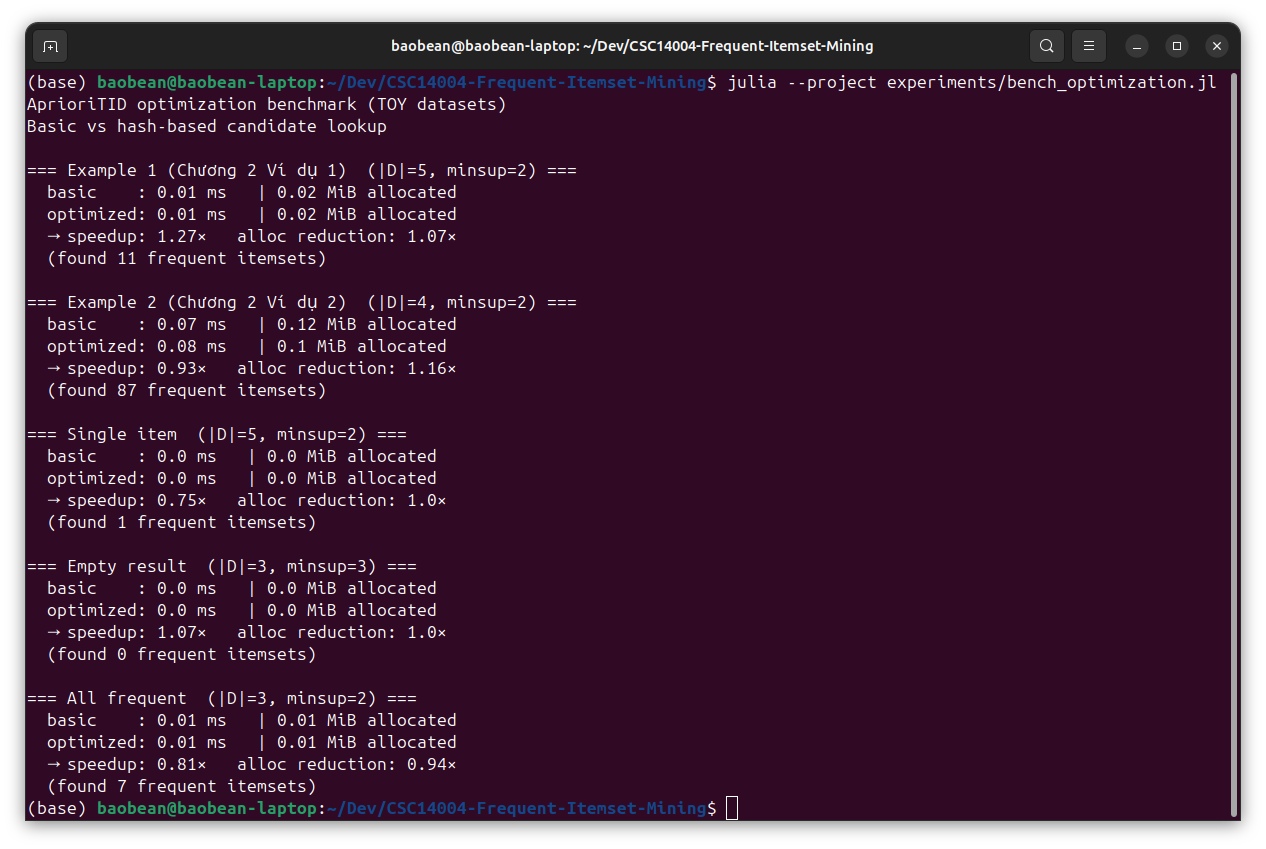
\includegraphics[width=0.92\linewidth]{Figures/03-Implementation/03-b-optimization.png}
    \caption{Kết quả đo biến thể \emph{cơ bản} và \emph{tối ưu} của \texttt{apriori\_tid} trên 5 bộ dữ liệu toy (minsup tuyệt đối in trực tiếp trong tiêu đề mỗi khối). Script sử dụng bộ đếm \texttt{@elapsed} và \texttt{@allocated} sau khi làm nóng JIT.}
    \label{fig:bench-opt-toy}
\end{figure}

\begin{table}[h!]
    \centering
    \caption{Tổng hợp tăng tốc và giảm cấp phát giữa hai biến thể trên 5 bộ dữ liệu toy.}
    \label{tab:bench-opt-toy}
    \begin{tabular}{l|c|c|c|c}
        \hline
        \textbf{Bộ dữ liệu} & \textbf{$|D|$} & \textbf{Tăng tốc} & \textbf{Giảm cấp phát} & \textbf{\#Itemsets} \\ \hline
        Ví dụ 1 (Chương 2) & 5 & $1.27\times$ & $1.07\times$ & 11 \\
        Ví dụ 2 (Chương 2) & 4 & $0.93\times$ & $1.16\times$ & 87 \\
        Single item        & 5 & $0.75\times$ & $1.00\times$ & 1  \\
        Empty result       & 3 & $1.07\times$ & $1.00\times$ & 0  \\
        All frequent       & 3 & $0.81\times$ & $0.94\times$ & 7  \\
        \hline
    \end{tabular}
\end{table}

\paragraph{Bình luận.} Trên dữ liệu toy, lợi thế của bảng băm tiền tố hầu như chưa hiện ra --- thậm chí ba trong năm trường hợp (\emph{Ví dụ 2}, \emph{Single item}, \emph{All frequent}) còn ghi nhận tăng tốc \emph{nhỏ hơn} 1$\times$ ($0.93\times$, $0.75\times$ và $0.81\times$), tức biến thể tối ưu chạy chậm hơn biến thể cơ bản. Nguyên nhân là $|C_k|$ trên các bộ này không bao giờ đủ lớn để chi phí dựng \texttt{Dict} tiền tố được hoàn vốn; với những bộ chỉ có vài ứng viên, một vòng quét tuyến tính của biến thể cơ bản còn rẻ hơn cả việc cấp phát một bảng băm. Tương tự, cấp phát hầu như đứng yên ($1.00\times$ ở \emph{Single item} và \emph{Empty result}) hoặc thậm chí xấu đi nhẹ ở \emph{All frequent} ($0.94\times$). Điểm sáng duy nhất là \emph{Ví dụ 1} với tăng tốc $1.27\times$ và \emph{Ví dụ 2} --- bộ dữ liệu đặc mà \autoref{cp:example} cố tình thiết kế để có $|\overline{C}_2| > |D|$ --- nơi cấp phát giảm $1.16\times$, gợi ý đúng hướng kỳ vọng: hiệu quả của tối ưu tỉ lệ thuận với mật độ và kích thước bài toán. Toy datasets không phải là môi trường để bảng băm tỏa sáng; phép đo có ý nghĩa phải thực hiện trên các bộ chuẩn (chess, mushrooms, retail, T10I4D100K), nơi \autoref{cp:experiment-evaluation} ghi nhận giảm cấp phát từ $1.45\times$ tới $35.7\times$.

\section{Kiểm thử và xác minh}
\label{sec:impl-tests}

Thư mục \texttt{tests/} là điểm vào kiểm thử đơn vị, được gom gọn thành ba file phẳng. File \texttt{tests/runtests.jl} đóng vai trò điểm vào trực tiếp (không còn là \emph{shim}) và nạp lần lượt các file test, đảm bảo lệnh bắt buộc của đề bài hoạt động:

\begin{minted}{bash}
julia --project tests/runtests.jl
\end{minted}

\subsection{Hai file kiểm thử tự động}

\begin{itemize}
    \item \texttt{test\_correctness.jl} --- kiểm thử \emph{theo bảng cố định} (fixture-driven): với mỗi bộ dữ liệu toy, file này chạy \texttt{apriori\_tid} và đối chiếu trực tiếp từng cặp (itemset, support) với file tham chiếu SPMF đã sinh sẵn trong \texttt{data/toy/spmf\_reference/}, đồng thời in ra tỉ lệ trùng khớp. Nhờ gộp kiểm thử đúng đắn và kiểm thử tham chiếu thành một mạch, file này là bằng chứng trực tiếp cho \emph{cả hai} yêu cầu (a) \emph{cài đặt cơ bản} và (b) \emph{tái tạo đúng kết quả với ví dụ tham chiếu}.
    \item \texttt{test\_io.jl} --- kiểm thử \texttt{read\_spmf}, \texttt{write\_spmf}, quy trình \emph{roundtrip} (đọc -- ghi -- đọc lại), tính sắp xếp itemset đầu ra và các trường hợp biên (file trống, dòng trống, khoảng trắng thừa). Đây là bằng chứng trực tiếp cho yêu cầu (d) \emph{định dạng vào/ra}.
\end{itemize}

Năm bộ dữ liệu toy, mỗi bộ có một mục đích kiểm thử riêng, được tóm tắt ở \autoref{tab:toy-datasets}.

\begin{table}[htbp]
    \centering
    \caption{Năm bộ dữ liệu toy dùng trong \texttt{tests/test\_correctness.jl}.}
    \label{tab:toy-datasets}
    \begin{tabular}{l|c|c|l}
        \hline
        \textbf{File} & $|D|$ & \textbf{minsup} & \textbf{Mục đích} \\ \hline
        \texttt{example1.txt}          & 5 & 2 & Ví dụ 1 (\autoref{cp:example}) --- 11 itemset \\
        \texttt{example2.txt}          & 4 & 2 & Ví dụ 2 (\autoref{cp:example}) --- 87 itemset \\
        \texttt{test\_single\_item.txt} & 5 & 2 & Mọi giao dịch chỉ có 1 item \\
        \texttt{test\_empty\_result.txt}& 3 & 3 & \textit{minsup} cao, không itemset nào phổ biến \\
        \texttt{test\_all\_frequent.txt}& 3 & 2 & Mọi tập con đều phổ biến \\
        \hline
    \end{tabular}
\end{table}

\subsection{Kết quả}

\autoref{fig:test-correctness} cho thấy toàn bộ hệ thống kiểm thử vượt qua: \textbf{106/106 = 100.0\%} kết quả khớp SPMF trên 5 bộ dữ liệu toy, và tổng số test đơn vị là \textbf{33/33 Pass}. Số \textbf{106} là tổng số (itemset, support) hợp lại của cả 5 bộ dữ liệu toy --- 11 + 87 + 1 + 0 + 7 = 106.

\begin{figure}[h]
    \centering
    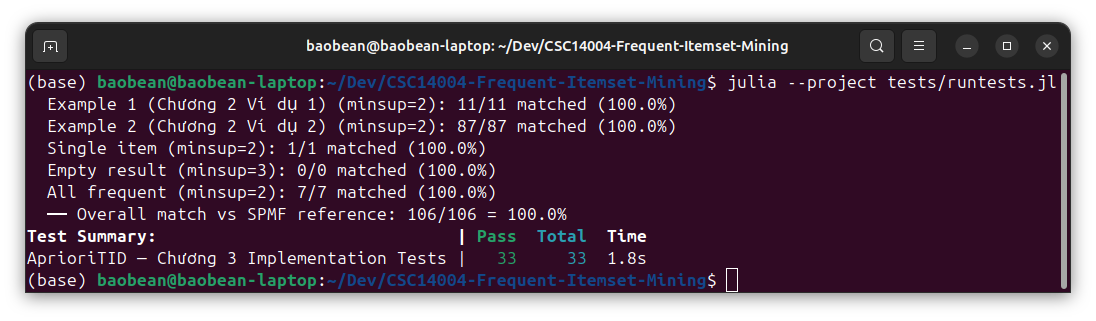
\includegraphics[width=0.92\linewidth]{Figures/03-Implementation/03-a-correctness.png}
    \caption{Kết quả chạy kiểm thử.}
    \label{fig:test-correctness}
\end{figure}
\chapter{Thực nghiệm và đánh giá}\label{cp:experiment-evaluation}

\chapter[Ứng dụng thực tế]{Ứng dụng thực tế}
\label{cp:application}

Chương này trình bày một ứng dụng thực tế của cài đặt AprioriTID ở \autoref{cp:implementation}: \textbf{phân tích giỏ hàng} (\textit{market basket analysis}) trên bộ dữ liệu giao dịch bán lẻ \textbf{Retail}. Mục tiêu là chuyển tập frequent itemset thu được thành các \textbf{luật kết hợp} (\textit{association rule}) có thể diễn giải được bằng ba độ đo --- \textit{support}, \textit{confidence} và \textit{lift} --- rồi rút ra một số quan sát có giá trị kinh doanh.

\section{Bài toán phân tích giỏ hàng}
\label{sec:mba-problem}

\paragraph{Phát biểu.} Cho một cơ sở dữ liệu giao dịch $D = \{t_1, t_2, \dots, t_n\}$, mỗi giao dịch là một tập con của tập item $I$. \textbf{Market Basket Analysis} đặt câu hỏi: \emph{những item nào có xu hướng được mua cùng nhau, và việc mua nhóm item $X$ có làm tăng xác suất mua nhóm item $Y$ hay không?} Câu trả lời được phát biểu dưới dạng các luật kết hợp
\[
    X \Rightarrow Y, \quad X, Y \subseteq I, \quad X \cap Y = \varnothing, \quad X \neq \varnothing, \ Y \neq \varnothing.
\]

\paragraph{Ba độ đo.} Mỗi luật $X \Rightarrow Y$ được đánh giá bởi ba đại lượng (\cite{AgrawalSrikant1994}):
\begin{align}
    \textit{support}(X \Rightarrow Y)    &= \frac{|\{t \in D : X \cup Y \subseteq t\}|}{|D|}, \\
    \textit{confidence}(X \Rightarrow Y) &= \frac{\textit{support}(X \cup Y)}{\textit{support}(X)}, \\
    \textit{lift}(X \Rightarrow Y)       &= \frac{\textit{confidence}(X \Rightarrow Y)}{\textit{support}(Y) / |D|}.
\end{align}
trong đó $\textit{support}(Z)$ là số giao dịch chứa tập $Z$. \textit{Support} đo tần suất tuyệt đối, \textit{confidence} đo xác suất có điều kiện $\Pr(Y \mid X)$, còn \textit{lift} đo mức tương quan so với giả thiết độc lập: $\textit{lift} = 1$ nghĩa là $X$ và $Y$ độc lập, $\textit{lift} > 1$ nghĩa là chúng đồng xuất hiện thường xuyên hơn ngẫu nhiên, và $\textit{lift} < 1$ nghĩa là chúng kị nhau.

\paragraph{Liên hệ với AprioriTID.} Việc sinh luật kết hợp tách làm hai bước kinh điển: (i) khai phá \textbf{tất cả frequent itemset} tại ngưỡng \textit{minsup} --- đây chính là đầu ra của AprioriTID; (ii) với mỗi itemset $F$ có $|F| \ge 2$, liệt kê mọi tập con riêng $X \subset F$ và xét luật $X \Rightarrow F \setminus X$. Vì $F$ và cả hai tập con $X$, $F \setminus X$ đều là itemset, giá trị \textit{confidence} được tính trực tiếp bằng phép chia hai số đếm đã có trong kết quả của AprioriTID mà không cần quét lại dữ liệu.

\section{Bộ dữ liệu Retail}
\label{sec:mba-data}

Retail là bộ giao dịch bán lẻ công khai của một siêu thị Bỉ, được phát hành bởi Tom Brijs và thường được dùng làm bộ chuẩn trong các nghiên cứu khai phá luật kết hợp (\cite{BrijsRetail1999}). \autoref{tab:retail-stats} tóm tắt các thông số cơ bản đo trực tiếp trên file \texttt{retail.txt}.

\begin{table}[htbp]
    \centering
    \caption{Thống kê cơ bản của bộ dữ liệu Retail.}
    \label{tab:retail-stats}
    \begin{tabular}{l|r}
        \hline
        \textbf{Thông số} & \textbf{Giá trị} \\ \hline
        Số giao dịch $|D|$       & 88\,162 \\
        Số item phân biệt $|I|$  & 16\,470 \\
        Độ dài giao dịch trung bình $\bar{w}$ & $\approx$\,10.3 \\
        Mật độ $\bar{w}/|I|$     & $\approx 6.3 \times 10^{-4}$ \\ \hline
    \end{tabular}
\end{table}

Khác với Chess hay Mushrooms, Retail là một bộ dữ liệu \textbf{rất thưa}: số lượng item gấp hàng ngàn lần độ dài giao dịch trung bình. Đặc điểm này làm cho phần lớn các item xuất hiện rất hiếm, và ngay cả tại ngưỡng \textit{minsup} tương đối thấp như $0.5\%$ ($\text{abs} \approx 441$), số frequent itemset vẫn giữ ở mức vài trăm --- rất phù hợp để minh họa việc sinh luật kết hợp mà không bị lạm phát đầu ra.

\section{Quy trình và cài đặt}
\label{sec:mba-pipeline}

Toàn bộ mã nguồn cho ứng dụng nằm trong thư mục \texttt{application/}, tách biệt với thư mục \texttt{src/} chứa thuật toán gốc:

\begin{itemize}
    \item \texttt{application/market\_basket.jl}: định nghĩa struct \texttt{AssociationRule}, hàm sinh luật từ tập frequent itemset \texttt{generate\_rules}, hàm \texttt{write\_rules\_csv} xuất luật ra CSV, và hàm tiện ích \texttt{top\_rules\_by} để trích top-$n$ luật theo một độ đo nhất định.
    \item \texttt{application/run\_retail.jl}: kịch bản CLI, đọc \texttt{retail.txt}, chạy AprioriTID ở \textit{minsup} chỉ định, sinh luật ở \textit{minconf} chỉ định và in bản tóm tắt ra stdout.
\end{itemize}

Cả hai file dùng lại trực tiếp các file trong \texttt{src/} bằng \texttt{include}, không lặp lại logic thuật toán.

\paragraph{Thuật toán sinh luật.} \texttt{generate\_rules} duyệt mọi itemset $F$ có $|F| \ge 2$ trong đầu ra của AprioriTID, rồi với mỗi $F$ liệt kê $2^{|F|} - 2$ tập con riêng không rỗng bằng \textbf{bitmask} --- với bit thứ $i$ bật nghĩa là item $F[i]$ thuộc tập tiền đề $X$, bit tắt nghĩa là thuộc hậu đề $Y$. Các support $\textit{sup}(X)$, $\textit{sup}(Y)$, $\textit{sup}(F)$ được tra trong dict \texttt{support\_of} xây sẵn từ kết quả AprioriTID, nên chi phí tổng thể chỉ là $O\!\left(\sum_{F} 2^{|F|}\right)$ phép tra. Vì các itemset mà AprioriTID trả về đều ngắn (trong thực nghiệm không quá $k=4$), chi phí sinh luật hoàn toàn không đáng kể so với chi phí FIM --- như sẽ thấy ở \autoref{sec:mba-results}.

\paragraph{Lệnh chạy.} Toàn bộ pipeline được gói trong một lệnh duy nhất:
\begin{minted}{text}
julia --project application/run_retail.jl 500 0.30
\end{minted}
trong đó \texttt{500} là \textit{minsup} tuyệt đối ($\approx 0.567\%$) và \texttt{0.30} là ngưỡng \textit{confidence} tối thiểu. Kết quả được ghi vào \texttt{experiment\_results/retail\_rules.csv}.

\section{Kết quả phân tích}
\label{sec:mba-results}

Với $\textit{minsup} = 500$ và $\textit{minconf} = 0.30$, cài đặt cho ra \textbf{468 frequent itemset} trong đó \textbf{283} có $|F| \ge 2$, và sinh ra \textbf{406 luật kết hợp} thoả mãn ngưỡng \textit{confidence}. Tổng thời gian chạy: 3549\,ms cho bước FIM và chỉ 0.2\,ms cho bước sinh luật --- xác nhận khẳng định rằng chi phí sinh luật gần như miễn phí khi đã có frequent itemset.

\subsection{Top luật theo confidence}

\autoref{tab:retail-top-conf} liệt kê 10 luật có \textit{confidence} cao nhất. Cả 10 luật đều có hậu đề là \emph{item 39} --- item phổ biến nhất trong Retail ($\textit{sup}(\{39\}) \approx 57\%$). Đây là hiện tượng kinh điển khi sinh luật không lọc theo \textit{lift}: một item có tần suất nền rất cao sẽ xuất hiện trong gần như mọi giao dịch, kéo theo \textit{confidence} của bất kỳ luật nào trỏ về nó đều xấp xỉ xác suất nền của chính nó.

\begin{table}[htbp]
    \centering
    \caption{Top 10 luật theo \textit{confidence} tại $\textit{minsup} = 500$, $\textit{minconf} = 0.30$.}
    \label{tab:retail-top-conf}
    \begin{tabular}{l|r|r|r}
        \hline
        \textbf{Luật} & \textbf{sup} & \textbf{conf} & \textbf{lift} \\ \hline
        $\{40, 49, 111\} \Rightarrow \{39\}$ & 0.0117 & 0.994 & 5.62 \\
        $\{40, 42, 111\} \Rightarrow \{39\}$ & 0.0058 & 0.992 & 5.61 \\
        $\{40, 49, 171\} \Rightarrow \{39\}$ & 0.0135 & 0.989 & 5.59 \\
        $\{40, 111\}      \Rightarrow \{39\}$ & 0.0197 & 0.989 & 5.59 \\
        $\{40, 372\}      \Rightarrow \{39\}$ & 0.0060 & 0.989 & 5.59 \\
        $\{49, 171\}      \Rightarrow \{39\}$ & 0.0174 & 0.988 & 5.58 \\
        $\{42, 171\}      \Rightarrow \{39\}$ & 0.0090 & 0.986 & 5.58 \\
        $\{49, 111\}      \Rightarrow \{39\}$ & 0.0154 & 0.986 & 5.58 \\
        $\{38, 49\}       \Rightarrow \{39\}$ & 0.0063 & 0.986 & 5.57 \\
        $\{40, 42, 171\}  \Rightarrow \{39\}$ & 0.0070 & 0.986 & 5.57 \\ \hline
    \end{tabular}
\end{table}

Mặc dù \textit{confidence} của cả 10 luật đều xấp xỉ $0.99$, \textit{lift} vẫn rơi vào khoảng $5.6$, nghĩa là xác suất xuất hiện của item 39 \emph{có điều kiện} gấp $5.6$ lần so với xác suất nền. Quan sát này cho thấy: trong Retail tồn tại một tập lõi $\{39, 40, 42, 48, 49, 111, 171\}$ với các item cực kỳ tương quan --- nhiều khả năng đây là các mặt hàng nhu yếu phẩm xuất hiện đồng thời trong phần lớn hoá đơn.

\subsection{Top luật theo lift}

\autoref{tab:retail-top-lift} cho một góc nhìn rất khác. Hai luật đứng đầu bảng ---
$\{16011\} \Leftrightarrow \{16012\}$ và $\{271\} \Leftrightarrow \{272\}$ --- có \textit{support} rất nhỏ ($< 1\%$), \textit{confidence} khiêm tốn, nhưng \textit{lift} cực lớn ($65.19$ và $16.51$). Các item trong các luật này hầu như chỉ xuất hiện cùng nhau: biết một item, xác suất thấy item kia tăng lên hàng chục lần.

\begin{table}[htbp]
    \centering
    \caption{Top 10 luật theo \textit{lift}. Các cặp song hướng ($A \Rightarrow B$ và $B \Rightarrow A$) được giữ nguyên để thấy sự bất đối xứng về confidence.}
    \label{tab:retail-top-lift}
    \begin{tabular}{l|r|r|r}
        \hline
        \textbf{Luật} & \textbf{sup} & \textbf{conf} & \textbf{lift} \\ \hline
        $\{16011\} \Rightarrow \{16012\}$ & 0.0074 & 0.495 & 65.19 \\
        $\{16012\} \Rightarrow \{16011\}$ & 0.0074 & 0.973 & 65.19 \\
        $\{271\}   \Rightarrow \{272\}$   & 0.0077 & 0.392 & 16.51 \\
        $\{272\}   \Rightarrow \{271\}$   & 0.0077 & 0.325 & 16.51 \\
        $\{37, 42\}   \Rightarrow \{39, 40\}$ & 0.0063 & 0.790 & 6.73 \\
        $\{49, 171\}  \Rightarrow \{39, 40\}$ & 0.0135 & 0.766 & 6.53 \\
        $\{42, 171\}  \Rightarrow \{39, 40\}$ & 0.0070 & 0.764 & 6.51 \\
        $\{40, 111\}  \Rightarrow \{39, 49\}$ & 0.0117 & 0.586 & 6.50 \\
        $\{37, 49\}   \Rightarrow \{39, 40\}$ & 0.0123 & 0.763 & 6.50 \\
        $\{42, 111\}  \Rightarrow \{39, 40\}$ & 0.0058 & 0.755 & 6.43 \\ \hline
    \end{tabular}
\end{table}

Quan sát \emph{bất đối xứng} giữa hai hướng là đáng chú ý. Cặp $\{16011, 16012\}$ có $\textit{conf}(16011 \Rightarrow 16012) = 0.495$ nhưng $\textit{conf}(16012 \Rightarrow 16011) = 0.973$. Điều này cho biết item 16012 gần như luôn được mua kèm 16011, nhưng không ngược lại --- một tín hiệu điển hình của quan hệ \emph{mặt hàng phụ kiện $\to$ mặt hàng chính} (chẳng hạn \emph{pin cho đèn pin}: có pin thì chưa chắc có đèn, nhưng có đèn thì thường có pin).

\subsection{Thảo luận kinh doanh}

Từ hai bảng trên có thể rút ra ba nhóm quan sát có giá trị ứng dụng thực tế:

\begin{enumerate}
    \item \textbf{Lõi nhu yếu phẩm.} Tập $\{39, 40, 42, 48, 49, 111, 171\}$ tạo thành một nhóm item đồng xuất hiện rất mạnh, cả về \textit{support} lẫn \textit{lift}. Trong thực tế, đây là các mặt hàng nên được bố trí sao cho khách hàng đi qua cả nhóm trong cùng một hành trình mua sắm, hoặc được gộp làm tiêu chí đánh giá \emph{độ đầy đủ} của một giỏ hàng trung bình.
    \item \textbf{Cặp phụ kiện $\to$ mặt hàng chính.} Các cặp \textit{lift} cao nhưng \textit{support} thấp (như $\{16011, 16012\}$, $\{271, 272\}$) gợi ý cơ chế \emph{gợi ý chéo} (\textit{cross-sell}): khi khách thêm 16012 vào giỏ, hệ thống có thể đề xuất kiểm tra xem có cần 16011 hay không, vì hai item gần như luôn đi đôi.
    \item \textbf{Cảnh báo bẫy confidence.} Nếu xếp hạng luật chỉ bằng \textit{confidence}, toàn bộ top bảng sẽ bị chiếm bởi các luật trỏ về item 39 --- một điều thực ra không mang thông tin gì (item 39 xuất hiện ở hầu hết giao dịch). Trong pipeline sản phẩm, việc chặn dưới \textit{lift} (chẳng hạn $\textit{lift} > 2$) là cần thiết để loại bỏ các luật trivial như vậy.
\end{enumerate}

\section{Nhận xét tổng quan}
\label{sec:mba-discussion}

Ứng dụng trên là một minh chứng đầy đủ cho luận điểm: \emph{AprioriTID không phải là đích đến, mà là bước trung gian}. Toàn bộ chi phí tính toán tập trung ở bước FIM (3549\,ms), còn bước sinh luật chỉ mất 0.2\,ms --- tỷ lệ gần $14\,000 \colon 1$. Điều này có hai hệ quả quan trọng:

\begin{itemize}
    \item Một lần chạy FIM đủ để thử nghiệm nhiều cấu hình $(\textit{minconf}, \text{top-}n)$ khác nhau mà không phải chạy lại thuật toán gốc. Trong notebook \texttt{notebooks/demo.ipynb}, đặc điểm này được tận dụng để so sánh phân bố luật tại nhiều mức \textit{minconf} trong vòng vài giây.
    \item Chiến lược tối ưu cho phân tích giỏ hàng nên tập trung vào phía FIM: giảm \textit{minsup}, tăng kích thước dữ liệu hay thay bằng thuật toán sinh tập phụ (\emph{closed hay maximal itemset}) đều tác động đến bước tốn kém này chứ không phải bước sinh luật.
\end{itemize}

Một hạn chế đáng lưu ý: AprioriTID trả về \textbf{tất cả} frequent itemset, bao gồm cả các itemset ``dư'' (supersets có cùng support với một subset của nó). Với Retail ở \textit{minsup} thấp hơn (ví dụ $100$), số itemset có thể vượt vài ngàn, và số luật sinh ra tăng theo hàm mũ theo $|F|$ lớn nhất. Trong các phiên bản tiếp theo, thay AprioriTID bằng một biến thể khai phá \emph{closed frequent itemset} (như CHARM, \cite{ZakiHsiao2002CHARM}) hoặc \emph{maximal frequent itemset} (như MAFIA, \cite{Burdick2001MAFIA}) sẽ thu gọn đầu ra mà không mất thông tin --- đây là hướng mở rộng tự nhiên cho ứng dụng này.


%%% Bibliography %%%
\renewcommand{\refname}{Tài liệu tham khảo}
\printbibliography[title={\refname},heading=bibintoc]

%%% Appendices: Work that *YOU* Developed %%%
% \appendix
% \input{Matter/08-Appendices}
% \input{Chapters/Appendices/00-AppendixA}
% \input{Chapters/Appendices/01-AppendixB}

%%% Annexes: Work that *YOU DID NOT* Develop %%%
% \input{Matter/09-Annexes}
% \input{Chapters/Annexes/00-AnnexA}

%%% Back Page %%%
% \input{Matter/10-Back-Page}

\end{document}